% This section consists of three parts: first, we present the use case and the challenges related to it, then we explain how the use case can be approached using \nthree reasoning and as a last part 
% we evaluate our implementation against an implementation which has been done earlier where \owl-DL reasoning and SPARQL querying was employed.
Below, we first introduce our use case -- a semantic nurse call system -- and discuss the technical challenges connected to it. We then explain how this use case can be tackled by applying
ontology reasoning and querying and present our implementation 
with \nthreelogic:
%.
%Our solution involves OWL RL reasoning using the reasoner EYE. We explain how 
We use \owl RL reasoning to be able to incorporate knowledge specified in an \owl ontology (ontology reasoning) and write extra rules to support decision 
trees (querying). We first perform the \owl RL reasoning by directly applying the rules specified on the Web site introducing this profile~\cite{OWLRL} and then add a preprocessing step to further improve performance.  
We compare both implementations with an implementation using \owl DL reasoning and SPARQL querying.

\subsection{Use case description}
Our use case is a semantic nurse call system in a hospital:
The system is aware of certain details about personnel and patients. % represented in an OWL-DL ontology.
Such information can include: personal skills of a staff member, staff competences, patient information, special patient needs, and/or the 
personal relationship between staff members and patients. 
Furthermore, there is dynamic information available, for example, the current location of staff members and their status (busy or free). 
When a call is made, the nurse
call system should be able to assign the best staff member to answer that call. The definition of this ``best'' person
varies between hospitals and can be quite complex. 
The system additionally controls different devices. If for example staff members enter a room with a patient, 
a light should be switched on; if they log into the room's terminal, they should have access to the medical lockers in the room. 
%Our use case is a nurse call system in a hospital.
The event-driven reasoning system for this use case has to fulfil certain requirements.
\begin{description}
\item[scalability] It should cope with data sets ranging from 1000 to 100,000 relevant triples (ie triples necessary to be included for the reasoning to be correct). 
Especially in bigger hospitals the number of staff members and patients and thereby also the amount of available information about those can be quite big. 
It is not always possible to divide this knowledge into smaller independent chunks as this data is normally full of mutual dependencies. 
\item[functional complexity] It should implement deterministic decision trees with varying complexities. The reasons to assign a nurse to 
a certain patient can be as manifold as the data. Previous work has shown that this complexity is not only theoretically possible but also desired by the 
parties interested in such a semantic system~\cite{accioontold}.
\item[configuration] It should support the ability to change these decision trees at configuration time. Different hospitals have different 
requirements and even in one single hospital those requirements 
can easily change due to eg an increase of available information or a simple change in the hospital's organizational concepts or philosophy.
\item[real-time] It should return a response within 5 seconds to any given event. Especially in such a delicate sector as patient care, seconds can make a difference. 
Even though a semantic nurse call system will not typically be employed to assign urgent emergency calls  through complex decision trees, 
a patient should not wait too long till his possibly pressing request is answered.
\end{description}
% The functional complexity requirement together with the configuration constraint motivate 
% the choice of a reasoning system which supports rules as these can be seen as the most natural way to 
% express decision trees. Even though a numerous amount of OWL DL reasoners support at least one rule format, 
% their reasoning is too slow to meet the scalability and the real-time constraint \cite{ORCA}. \todo{that is the paper used for the first part of this section, so remove reference!}
% Therefore, we chose a rule-based solution. 
%Especially the last argument motivates us to solve the described problem using semantic web technologies as they natively fulfill the semantics requirement.



 
%\subsection{Implementation} 
% To keep the benefits of an OWL-DL based implementation in a scalable and real-time way, we propose a rule-based solution.
% By using OWL 2 RL rules and resolution instead of classical tableaux reasoning, we can significantly decrease reasoning times and still cover a major subset
% of OWL 2. This approach benefits from the high performance of rule based reasoners. 
% Even for bigger datasets the reasoning times are still faster than with the OWL-DL based approach. %very fast, as we will see later in this paper.  %and is able to reason very fast even over large datasets. 
% %Because of its high performance (see benchmarks mentioned in \cite{eyepaper}), we chose the EYE reasoner for our purposes. As the reasoner is 
% %able to cope with large datasets, our approach meets 
% Also, complex decision trees can directly be implemented in rules. %, as those form the most natural 
% As rules are the most natural representations of such trees, 
% it is easy for a user to understand and change certain priorities 
% or to configure new rules. A further advantage of our approach is that all logic is represented in one single way. Instead of
% OWL plus SPARQL, we can implement the business case by only employing Notation3 Logic (N3). With the aforementioned system, we can meet all necessary requirements.
%We use OWL 2 RL rules to reason about the ontology
% -- syntactically represented Turtle and therefore compatible with \nthree{} -- and add custom rules do model the decision tree. 
% Below, we explain our solution in detail.

\subsection{Benefits of a semantic approach}
There are several options to implement a nurse call system as described above. Following a more classical approach, the system could be written in 
an object-oriented programming language 
such as Java or C++. An implementation like this can easily fulfil the real-time and scalability constraints.
But such systems are traditionally hard-coded: they are implemented for a specific use case, and even though 
they might be able to support the required functional complexity, this implementation would be static. The possibility to configure complex decision trees
as postulated by the complexity requirement is rather hard to fulfil using traditional programming. Even more difficult to satisfy is the semantic requirement:
most object oriented languages do not support enough logic to ``understand'' the available information. Knowledge must be stated explicitly, 
as even simple connections between statements such as ``\textit{nurse x has location y}'' and ``\textit{y is location of nurse x}'' cannot be found easily.

Especially the last argument motivates us to solve the described problem using Semantic Web technologies as they natively fulfil the semantics requirement.
Knowledge can be represented in an OWL ontology which is understood by OWL DL reasoners. % such as for example Pellet \cite{Pellet}. % or HermiT \cite{hermit}.
Complex decision trees can be handled by subsequent SPARQL queries. It is easy to add new queries or to change the order of existing queries 
and to thereby accommodate for the configuration constraint.
But our tests (see Section~\ref{ev} below) have shown that such systems inherently are not fast and reliable enough to fulfil the scalability and real-time requirements.
For bigger amounts of data or too complex decision trees, the reasoning times of traditional OWL DL reasoners grow exponentially, which is not scalable.

To keep the benefits of an OWL DL based implementation in a scalable and real-time way, we propose a rule-based solution. % using \nthreelogic.
 By using rules to reason over the ontology
%  and 
%  resolution instead of classical tableaux reasoning, 
 we can significantly decrease reasoning times.
%  and still cover a major subset
%  of OWL 2. This approach benefits from the high performance of rule based reasoners. 
% Even for bigger datasets the reasoning times are still faster than with the OWL DL based approach. %very fast, as we will see later in this paper.  %and is able to reason very fast even over large datasets. 
% %Because of its high performance (see benchmarks mentioned in \cite{eyepaper}), we chose the EYE reasoner for our purposes. As the reasoner is 
% %able to cope with large datasets, our approach meets 
Complex decision trees can directly be implemented in rules. %, as those form the most natural 
 As rules are the most natural representations of such trees, 
 it is easy for a user to understand and change the priorities of different assignments 
 or to configure new rules. A further advantage of our approach is that all logic is represented in one single way. Instead of
 OWL DL reasoning plus SPARQL querying, we can implement the use case by only employing \nthreelogic. With the aforementioned system, we can meet all necessary requirements.
% 
% % 
% 
% 
% 
% In a first attempt it has been tried to approach this use case using OWL-DL reasoning:
% The knowledge can be expressed using an OWL DL ontology und interpreted by OWL DL reasoners such as for example Pellet \cite{Pellet}. % or HermiT \cite{hermit}.
% Complex decision trees can be handled by subsequent SPARQL queries. It is easy to add new queries or to change the order of existing queries 
% and to thereby accommodate for the configuration constraint.
% But our tests (see Section~\ref{ev} below) have shown that such systems inherently are not fast and reliable enough to fulfil the scalability and real-time requirements.
% For bigger amounts of data or too complex decision trees, the reasoning times of traditional OWL DL reasoners grow exponentially, which is not scalable.
% 
%Given the shortcomings of the solution using OWL DL reasoning and SPARQL it makes sense to implement the solution following another approach. 
%Below, we describe how we used \nthreelogic to solve the problem.
Below, we describe the details of our solution.

\subsection{OWL RL in \nthree}\label{owlrln3}
If we use a traditional OWL DL reasoner like for example Pellet \cite{Pellet} or HermiT \cite{hermit} to reason over an existing ontology 
this reasoner 
natively understands the concepts which are part of the OWL DL profile and applies 
different inference steps in a predefined order to derive new knowledge. % applying a tableaux algorithm (see for example \cite[chapter 2]{dl}).
%  
% 
% 
% Every \owl ontology has a representation in \rdf/XML (see also Section~\ref{rdfandowl}). This can easily be translated to \rdf/Turtle which then is syntactically compatible with 
% \nthree. 
% 
% 
% 
% % General explanation: ABox, TBox. representation of the knowledge against reasoning.
% % 
% % Say  that N3 is interesting because we can make rule-producing rules.
% % 
% % 
% Traditionally, reasoning over OWL ontologies was performed by description logic based reasoners using (variants of) the tableaux algorithm.
% Prominent examples of such reasoners are Pellet \cite{Pellet} and HermiT \cite{hermit}. 
% Both support---as others of their kind---the full OWL DL profile. 
%As the OWL-DL profile is very expressive and contains a huge variety of different concepts and the complexity of the related reasoning,
As OWL DL is very expressive and contains a huge variety of different concepts, OWL DL reasoners perform rather slow in comparison with, for example, rule-based reasoners. 
% which mostly only
% apply one kind of inference step.
The OWL 2 profiles \cite{OWLRL} aim to overcome this gap 
by defining less expressive
but still powerful subsets of OWL DL. One of these profiles is OWL RL, which was designed to enable rule-based reasoners to cope with OWL ontologies. 

For each OWL concept which forms part of the RL profile the specification lists one or more rule %which can be written in a rule language with at least the expressiveness of Datalog~\cite{datalog}
which can be used to draw conclusions from it. These rules written in a generic \rdf rule language with the expressiveness of Datalog~\cite{datalog} -- ie simple rules which do not allow functions 
or new existential variables in their conclusion
-- and can be translated to 
every rule language being at least equally expressive. 
These rules then either directly act on the syntactical representation of the ontology -- this is what we do in our implementation -- 
or on its translation to the input format of the rule language -- this is for example done by OWLim \cite{owlim} and Oracle's RDF Semantic Graph \cite{oracle}.
%The advantage of specifying rules in a format which is compatible with \rdf and reason directly on the ontology is that it remains transparent which rules are used and 
By using \nthree which is compatible with \rdf/Turtle we make sure that the reasoning performed does not depend on the way the triples are translated to an internal format. 
In that sense we are reasoner independent. This approach furthermore makes it easier for the data consumer to understand or choose which rules are applied.  
% 
% if that is not \rdf.
% %and have been translated and used in different formats and by different reasoners like 
% %as for example the reasoners 
% An example for the latter are the reasoners OWLim \cite{owlim} and Oracle's RDF Semantic Graph \cite{oracle} which both use an internal rule-language 
% for reasoning not directly related to \rdf.
% %  In these last two reasoners, as well as most other reasoners we are aware of, the rules are 
% %  written and stored in an internal rule format which makes it difficult for the user to understand the derivations made or to choose which concepts should be supported by a a reasoner in a 
% %  specific use case.
% %Of course these rule language needs to act on the specific 
% As a consequence the 
 
% In our implementation we use \nthree rules: As the \rdf representation Turtle is fully compatible with \nthree, the syntactic representation of the ontology can directly serve as input 
% for the reasoner. The rules can be written in the same language and thus be exchanged between different reasoners. 
%
% The idea here is that the \rdf representation of the ontology serves as input for the reasoner and the derivations which can be made based on the semantics of the different 
% OWL concepts are supported by rules. These rules need  to be specified in the rule language. % and the website
%We started from an OWL-DL ontology which was used to 
%Possible data which can be processed by our system  
%The ACCIO Ontology
% 
% To be able to support OWL 2 RL reasoning in N3 we used the OWL 2 RL/\rdf rules as listed on the corresponding website~\cite{OWLRL}. 
% Where possible, we made use of existing N3-translations of these rules as provided by EYE~\cite{EYEowl}. 
% Missing concepts were added. 
% The knowledge about patients, staff and the hospital set-up in general was specified using the ACCIO  ontology\footnote{Available at: \url{https://github.com/IBCNServices/
% Accio-Ontology/tree/gh-pages}}\cite{accioont}.
% Even though this ontology is designed for OWL-DL reasoning, the limitation to OWL RL had no impact for 
% our specific use case. %, all derivations needed to cope with the desired decision trees were supported by OWL RL. 
% 
% 
\begin{lstlisting}[
  float=t,
  caption={OWL-RL rule for \texttt{rdfs:subClassOf} class axiom in N3.},
  label=lst:subclass]
§\textcolor{gray}{@prefix rdfs: <http://www.w3.org/2000/01/rdf-schema\#>.}§
§\textcolor{gray}{@prefix rdf: <http://www.w3.org/1999/02/22-rdf-syntax-ns\#>.}§

{?C rdfs:subClassOf ?D. ?X a ?C} => {?X a ?D}.
\end{lstlisting}
% To illustrate the idea of using rules for OWL reasoning, we give a small example: Listing~\ref{lst:subclass} shows 
% the class axiom rule\footnote{The rule is the N3 version of the cax-sco rule in Table 7 on the OWL 2 Profiles website~\cite{OWLRL}.} which is needed 
% to deal with the rdfs concept
%  \verb!subclassOf!. For convenience we omit the prefixes in the formulas below. The empty prefix refers to the ACCIO ontology, 
%  \verb!rdf! and \verb!rdfs! have the same meaning as in Listing~\ref{lst:subclass}. Consider that we have the following T-Box triple stating that the class \verb!:Call!
%  is 
%  a subclass of the class \verb!:Task!:
%  %If the ontology contains the triples
% \begin{equation}
%  \verb!:Call rdfs:subClassOf :Task.! \label{1}
% \end{equation}
% If the A-Box contains an individual which is member of the class \verb!:Call!
% \begin{equation}\verb! :call1 a :Call.! \label{2}\end{equation}
% %a rule based reasoner can use the rule given in listing \ref{lst:subclass} to conclude 
% an OWL DL reasoner would make the conclusion that the individual also belongs to the class \verb!Task! 
% \begin{equation}
%  \verb!:call1 a :Task.! \label{3}
% \end{equation}
% Our rule in Listing \ref{lst:subclass} does exactly the same: as Formula~\ref{1} and Formula~\ref{2} can be unified with the antecedence of the rule, a reasoner derives
% the triple in Formula~\ref{3}. Other concepts can be handled similarly.
% 
%In a first attempt to solve the above-mentioned problem we used a direct translation of 
% How this can be done is explained in the specification of OWL RL~\cite{OWLRL} where the concrete OWL 2 RL/\rdf rules
% are listed in a generic rule language. %as listed on the corresponding website. 
% 
% As \nthree is compatible with Turtle -- one representation format of \rdf -- 
%
%Where possible, we made use of existing N3-translations of these rules as provided by 

Below, we explain OWL RL reasoning in \nthree on a concrete example taken from our use case.
The OWL RL rule we show as well as the other used in our implementation are taken from the EYE website~\cite{EYEowl}. %, where needed, additional rules were added following the 
Knowledge is represented using the ACCIO ontology \cite{accioont} which will be further described in section \ref{ont}.
% The results of this 
% implementation were already promising \cite{arndt_ruleml_2015},\todo{replace reference} but for larger data sets the reasoning took multiple minutes and, thus, did not meet the requirements claimed above. 
% We explain the idea behind these OWL RL rules in \nthree %and how they can be improved
% using
% %We start with 
% an example:
Listing~\ref{lst:subclass} shows 
the class axiom rule\footnote{The rule is the N3 version of the cax-sco rule in Table 7 on the OWL 2 Profiles website~\cite{OWLRL}.} which is needed 
to deal with the \rdf{}s concept  \verb!subclassOf!.
For convenience we omit the prefixes in the formulas below. The empty prefix refers to the ACCIO ontology, 
 \verb!rdf! and \verb!rdfs! have the same meaning as in Listing~\ref{lst:subclass}. Consider that we have the following %TBox 
 triple stating that the class \verb!:Call!
 is 
 a subclass of the class \verb!:Task!:
\begin{equation}
 \verb!:Call rdfs:subClassOf :Task.! \label{1}
\end{equation}
If the ontology %ABox 
contains an individual which is member of the class \verb!:Call!
\begin{equation} \verb! :call1 a :Call.! \label{2}\end{equation}
an OWL DL reasoner would make the conclusion that the individual also belongs to the class \verb!Task!: 
\begin{equation}
 \verb!:call1 a :Task.! \label{3}
\end{equation}
Our rule in Listing \ref{lst:subclass} does exactly the same: as Formula~\ref{1} and Formula~\ref{2} can be unified with the antecedent of the rule, a reasoner derives
Formula~\ref{3}. 
%


\subsection{Decision trees}
%REMARK: Still not sure whether we need this section?
%The decision trees which have to be implement
%As mentioned above, decision trees as needed in for real life use cases can be quite complex. 

%Depending on the amount of available information, decision trees for nurse call systems can be quite complex. The ACCIO ontology 
%supports a huge variety of different concepts. %It is possible to model the profile of a patient (among others the 
 
The ACCIO ontology provides the user with a huge variety of concepts which can, eg be used to describe patients (social background, needs, disease), 
staff members (skills, relationships to patients), and situations (locations of persons, states of devices). If all this information is actually available, decision trees
can use all of it and be therefore quite complex. Here, we provide two simple rules which could be part of such a tree and we explain how these rules can
be modified depending on the needs of an individual hospital.
 
 \begin{lstlisting}[
  float=t,
  caption={Rule assigning a preference value to a staff member with status "free" who is close to the call-location. },
  label=lst:ex]
§\textcolor{gray}{@prefix : <http://ontology/Accio.owl\#>.}§
§\textcolor{gray}{@prefix rdf: <http://www.w3.org/1999/02/22-rdf-syntax-ns\#>.}§

{
  ?c rdf:type :Call.
  ?c :hasStatus :Active. 
  ?c :madeAtLocation ?loc. 
  ?p :hasRole [rdf:type :StaffMember].
  ?p :hasStatus :Free.
  ?p :closeTo ?loc.
}
=>
{
  (?p ?c) :assigned 200.
}.
\end{lstlisting}
 
Listing~\ref{lst:ex} shows a rule which, given an active call, assigns a staff member with a certain preference to that call. 
As explained in Section~\ref{prn3}, \nthree reasoners can be used goal-driven: The reasoner outputs all instances of the result of a filter rule which it can derive 
based on the input at hand, in our example all combinations of persons assigned to calls and their preference number. 
By using built-in functions we can now search for the highest or lowest preference number.
%By using built-in functions, such a filter can find the minimum or maximum values for certain conditions.
% Using built-in functions we can write a query which searches 
% % The EYE reasoner works 
% % with filter rules (queries), 
% %This makes it easy to search
% for the assignment of a staff member with the lowest or highest number. 
In our example, lower numbers mean higher preferences. The antecedence of the given rule contains certain constraints: the active call is made on a certain location and
there is a staff member, who is currently free and close to that location. In such a case, our rule assigns the number 200 to the combination of call and staff member.

\begin{lstlisting}[
  float=t,
  caption={Rule assigning a preference value to a busy staff member who has the needed skills to answer the call. },
  label=lst:ex2]
§\textcolor{gray}{@prefix : <http://ontology/Accio.owl\#>.}§
§\textcolor{gray}{@prefix rdf: <http://www.w3.org/1999/02/22-rdf-syntax-ns\#>.}§

{
  ?c rdf:type :Call.
  ?c :hasStatus :Active.
  ?c :hasReason [rdf:type :CareReason].
  ?p rdf:type :Person.
  ?p :hasStatus :Busy.
  ?p :hasRole [rdf:type :StaffMember].
  ?p :hasCompetence [rdf:type :AnswerCareCallCompetence].
}
=>
{
  (?p ?c) :assigned 100.
}.
\end{lstlisting}



Listing~\ref{lst:ex2} displays another rule: here, the reason of the active call is known. We have a staff member who has the required 
skills to answer that kind of calls, but this staff member is currently busy. Our rule assigns the number 100 to this
combination of call and staff member. This means, in our current decision tree, we prefer this assignment to the one described by Listing~\ref{lst:ex}.

Now, it could be, that another hospital has different priorities. Imagine for example that in this new hospital, no busy staff should be called 
if there is still a free staff member available, regardless of the reason of the call. We could easily adapt our decision tree by simply changing the assignment number 
of one of the rules. If we replace the triple \[\verb! (?p ?c) :assigned 100.!\] in line 15 of Listing \ref{lst:ex2} by the triple \[\verb! (?p ?c) :assigned 300.!\]
the reasoner would prefer the assignment expressed by Listings \ref{lst:ex} to~\ref{lst:ex2}.

 
Similarly, we can add extra conditions to the rules. Currently, the rule in listing \ref{lst:ex2} does not take the location of the staff member into account. We can
change that by only adding the triples 
\[ \verb!?c :madeAtLocation ?loc. ?p :closeTo ?loc.!\]
to the antecedence of the rule. To give this new rule a higher priority than the existing one, we would again only have to change the assigned number in the consequence.
Rules with the same number are treated equally.



\subsection{Improving performance by pre-producing TBox-rules}\label{reasoning}

In a first attempt we implemented the reasoning and querying as explained above and could already perform better than the solution employing \owl reasoning and SPARQL querying 
(see Section~\ref{ev} below). 
However, we could not meet the requirements mentioned above: our reasoning did not scale well and and it did not fulfil the real-time constraint. 
For that reason, we used an optimisation strategy 
which takes advantage of a specific feature of \nthree: 
In \nthree it is possible to write and apply rules having new rules in their consequences, we call these \emph{rule-producing rules}. 

% The key idea of our approach is now that there 
% is some knowledge in the ontology which does not change at execution time of the reasoning system: The fact that a call is a kind of task as specified in Formula~\ref{1} will not be changed 
% by the fact that for example a nurse is moving from one room to another.


% and have been translated and used in different formats and by different reasoners like for example 
%  OWLim \cite{owlim} and Oracle's RDF Semantic Graph \cite{oracle}. In these last two reasoners, as well as most other reasoners we are aware of, the rules are 
%  written and stored in an internal rule format which makes it difficult for the user to understand the derivations made or to choose which concepts should be supported by a a reasoner in a 
%  specific use case.
% Various implementations make use of 
% the OWL 2 RL/\rdf rules as proposed in the specification, among them
%  OWLim \cite{owlim} and Oracle's RDF Semantic Graph \cite{oracle}. 
% As most other implementations we are aware of, these reasoners support their own rule format, 
% and optimizations are done internally using
% the underlying programming language. 
% We propose an optimization which can be done in the logic itself by performing an extra reasoning step.
% We are thereby independent of a specific reasoner.

To better understand how we can benefit from rule-producing rules we go back to the above example: 
By unifying the antecedent of the rule in Listing~\ref{lst:subclass} with Formulas~\ref{1} and \ref{2} we could derive Formula~\ref{3}.
But this unification is rather expensive: The antecedent contains three different variables occurring 
in two different triples which have to be instantiated with the data of the ontology. % and this unification needs to be done whenever a new call is made.
%Our idea is now to make these unifications as early as possible and not
%We use rule-producing rules to do a pre-reasoning step: 
%Our solution now distinguishes between static and dynamic data: 
While information as stated in 
Formula~\ref{2} can change -- patients will make new calls -- statements as Formula~\ref{1} can be considered as fixed.
% and we can thus already perform this part of the unification before 
% we encounter 
The terminology does not change during the reasoning process,
calls are tasks for our ontology. %Our solution makes use of this observation: 
%The ontology contains more triples like Formula~\ref{1} which specify the terminology: % as for example classes and their relationships among each other.
Triples as the above specifying the terminology of an DL ontology are known as the TBox \cite[ch. 1]{dl}. 
%A description logic ontology consists of two parts: the TBox and the ABox \cite[chapter 1]{dl}.
% What is valid for Formula~\ref{1} also counts for 
% the other triples specifying the terminology. 
%In description logic these kinds of triples together form the TBox \cite[chapter 1]{dl}, the terminological knowledge.
Here the broader concepts (classes) and their relationships among each other are specified  
while the ABox contains triples over individuals.
We consider the
TBox as static knowledge which can be used for pre-processing. The idea of our solution is to do as much unification as possible before dealing with (possibly) dynamic data. 
We produce more specialized rules, in the case mentioned above, for example the rule
%
\begin{equation} 
\verb!{?X a :Call.} => {?X a :Task.}.!
\label{4}
\end{equation}
which will derive for every new call, that it is also a task, just as the rule in Listing~\ref{lst:subclass} does.

%Below we describe how we produce specialized rules based on the concepts present in the ontology's TBox, 
%with 
Below we describe our implementation.
% Reasoning in EYE can be considered as a single  process, having as input all necessary files representing the knowledge 
% (ie the necessary ontologies, data, and rule-files), and a query-file that filters the output of the reasoning result.
%We use the EYE reasoner and
We perform two steps:
\begin{enumerate}
 \item Produce a grounded copy of the  TBox. 
 \item Use rules to translate the grounded TBox into specialized rules.
\end{enumerate}

The need of the first step has to do with the fact that 
OWL ontologies represented in \rdf often use \emph{structural blank nodes} (see Section~\ref{strucblanks}):
As for example the union or the intersection of two classes cannot directly serve as subject of object in a triple, an anonymous blank node is normally introduced in such cases to
represent the construct.
% Blank nodes are for example used to represent the anonymous class  
% for concepts as for example intersection or union of classes ontology can contain anonymous classes represented by blank nodes.
Used in rules, 
these blank node class names have a 
limited scope (remember the examples from Section~\ref{existentials}). It is therefore difficult to use them to reference the same class in different rules. 
We will give a more elaborate explanation in the next section. 
After that we will describe the translation step in more detail.



\subsubsection{Grounding the Ontology}
\begin{lstlisting}[
  float=t,
  caption={ACCIO example: a call is both, a patient task and an unplanned task. },
  label=task]
§\textcolor{gray}{@prefix : <http://ontology/Accio.owl\#>.}§
§\textcolor{gray}{@prefix owl: <http://www.w3.org/2002/07/owl\#>.}§
§\textcolor{gray}{@prefix rdf: <http://www.w3.org/1999/02/22-rdf-syntax-ns\#>.}§
§\textcolor{gray}{@prefix rdfs: <http://www.w3.org/2000/01/rdf-schema\#>.}§

:Call  rdfs:subClassOf [ 
                       rdf:type owl:Class ;
                       owl:intersectionOf ( 
                                     :PatientTask
                                     :UnplannedTask
                                   )
                       ].
\end{lstlisting}


Before translating the TBox into rules we have to replace all blank nodes by \uris or literals. To understand the reason for this skolemization step, 
consider Listing~\ref{task}.
The example contains triples which further describe the class \texttt{:Call} from Formula~\ref{2}.
A call is a patient task and an unplanned task, or to be more specific:
There exists an anonymous class of which the class \texttt{:Call} is a subclass and which is the intersection of 
the classes \texttt{:PatientTask} and \texttt{:UnplannedTask}. 
%Even though \nthree supports rules which contain blank nodes,
It is exactly this anonymous class which causes problems. As we discussed in Section~\ref{strucblanks}
blank nodes are not simply variables, they are variables with an implicit existential quantifier and a specific scope. 
If we take the triple
\begin{equation}
 \texttt{:Call rdfs:subClassOf \_:y.}
\end{equation}
from line 6 of Listing~\ref{task}\footnote{Remember that \texttt{[ ]} stands for a ``fresh'' blank node, we chose to name it \texttt{\_:y} to make it easier to refer to it.}
and try to construct a rule from it in an analogous way as we did with Formula~\ref{1} and its resulting Rule~\ref{4} we would most probably come up with something like: 
%Being unlabelled, the blank node can be referred by an arbitrary new blank node name. A translation as done in Formula~\ref{4} would result in a rule like:
\begin{equation}
\verb!{ ?X a :Call. } => { ?X a _:y.}.! 
\label{newblank}
\end{equation}
But here the blank node \texttt{\_:y} is quantified in the consequence of the rule, in \nthree Core Logic this translates to:
\begin{equation}\tag{\ref{newblank}'}
 \forall\texttt{x: <type(x,Call)>}\rightarrow \texttt{<}\exists\texttt{y: type(x,y)>}
\end{equation}
This rule means, that every instance of the class \texttt{:Call} is also instance of \textit{some} other class. 
This knowledge can already be derived from Formula~\ref{4} where we have an example of such a class. 
% 
% and does 
% not have much influence 
% on further reasoning. And even if the blank node in Listing~\ref{task} would be labeled by, for example, \texttt{\_:intersection1} a new rule
% \begin{equation}
% \verb!{ ?X a :Call. } => { ?X a _:intersection1.}.! 
% \label{union}
% \end{equation}
% would have no other meaning than Formula~\ref{4} as in \nthree the scope of a blank node is always only the graph, i.e. the curly brackets \texttt{\{ \}}, 
% in which it occurs  \cite{Notation3, arndt_ruleml_2015}. 
With the local scoping of the blank node in the consequence of the rule, it is impossible to make the connection  between the class mentioned in the rule and the  
%The consequence of the rule would not refer to our 
intersection class of patient tasks and unplanned tasks by using blank nodes. We need to choose a constant representing the intersection class mentioned in Listing~\ref{task} 
which does not not change its scoping when used in the consequence of the rule. 

As \owl ontologies use a lot of such structural blank nodes which here can be understood as anonymous classes, we perform a grounding step.
Our implementation uses the EYE reasoner which provides the option to obtain a skolemized version of any input
\nthree file(s). 
The switch \verb!--no-qvars! replaces every blank node by a unique skolem \iri following the naming convention as described in the \rdf specification \cite{rdf}.
It additionally makes sure that equally named blank nodes only get assigned the same skolem \iri if they actually refer to 
the same thing. Producing a grounded version of the ontology enables us in further reasoning steps to use the 
new identifiers for (formally) anonymous classes in different rules.

\subsubsection{Translation Step}

 \begin{lstlisting}[
  float=t,
  caption={Rule producing new rule for every occurrence of \texttt{rdfs:subClassOf}; based on the \texttt{rdfs:subClassOf} class axiom of Listing~\ref{lst:subclass}.},
  label=lst:subclass2]
§\textcolor{gray}{@prefix rdfs: <http://www.w3.org/2000/01/rdf-schema\#>.}§
§\textcolor{gray}{@prefix rdf: <http://www.w3.org/1999/02/22-rdf-syntax-ns\#>.}§

{?C rdfs:subClassOf ?D.} => {{?X a ?C.}=>{?X a ?D.}.}.
\end{lstlisting}



As explained above, the next step after having produced a grounded version of the ontology's TBox is to produce the new specialized rules. 
Here we use rule-producing rules. %, we make use of a property of Notation3:
%we use rules can not only be applied to derive new triples but also to derive new rules. 
To understand the idea, consider the following example: 
%We explain the 
\begin{multline}\notag
 \texttt{\{}\underbrace{\texttt{:Call rdfs:subClassOf :Task.}}_{\text{\normalsize satisfied ontology triple(s)}} \texttt{\}}\\\texttt{=>\{}\underbrace{\texttt{\{?X a :Call\}=>\{?X a :Task.\}.}}_{\text{\normalsize produced new rule(s)}}\texttt{\}.}
 \end{multline}
%
Just as simple rules enable the reasoner to derive new triples from the fact that its antecedent is fulfilled, the rule above, applied on Formula~\ref{1}, derives a new rule, namely 
Formula~\ref{4}.
Nevertheless, the rule as stated above is too specific to be used for our purpose: if we already knew that the ontology contained the triple in Formula~\ref{1} we could also 
write the rule in Formula~\ref{4} directly instead of writing a rule which will surely produce it. Our rule needs to be more general as we want to handle 
all \texttt{owl:subclassOf} triples in that same way and always produce a rule 
similar to the rule expressed in Formula~\ref{4}. This more general rule can be found in Listing~\ref{lst:subclass2}.  Applied on Formula~\ref{1} the variable \texttt{?C} gets unified with 
the \uri \texttt{:Call} and the variable \texttt{?D} gets unified with \texttt{:Task}, thus, Rule~\ref{4} can be derived. Similarly, an application of the rule in 
Listing~\ref{lst:subclass2} on
triple 
\[
 \verb!:UnplannedTask rdfs:subClassOf :Task.!
\]
results in a new rule 
\[
 \verb!{?X a :UnplannedTask.} => {?X a :Task.}.!
\]

The same principle can be applied for other OWL concepts. Listing~\ref{list} shows a
rule\footnote{The rule is motivated by the cls-int2 rule in Table 6 on \cite{OWLRL}.} which handles the concept \texttt{owl:intersectionOf}. 
Note that this rule uses a built-in predicate of Notation3, \texttt{list:in}. A triple using \texttt{list:in} as a predicate is true  if and only if 
the object is a list and the subject is an entry of that list. 
If we apply this rule to the (now skolemized) intersection expressed in Listing \ref{task}
\begin{multline}\notag
\texttt{:InterClass1 owl:intersectionOf}\\\texttt{ (:PatientTask :UnplannedTask ).}
\end{multline}
  
\noindent two rules will be produced by that:  
\[\texttt{\{?x a :InterClass1\} => \{?x a :PatientTask.\}.}\]
\begin{center}
and
\end{center}
\[\texttt{\{?x a :InterClass1\} => \{?x a :UnplannedTask.\}.}\]

The above example illustrates how useful it is that Notation3 treats lists as first-class citizens and does not rely on reification here (see Sections \ref{strucblanks} and \ref{core}). 
% another useful property of Notation3: 
% Notation3 treats lists themselves, not only their reified version, as elements of the language.
There are many built-in predicates 
which enable the user to write 
clear rules operating on lists. For working with OWL ontologies this is a real advantage as lists are normally used
together with many OWL concepts 
like the above \texttt{owl:intersectionOf} or 
for example \texttt{owl:unionOf}.

If we apply the rule-producing rules as filter rules (see Section \ref{prn3}) in an \nthree reasoning run having the ground version of the ontology's TBox as input, the reasoner
produces a file only containing our specialized rules
% To produce new rules by applying the rules described above, the rule-producing rules have to be applied as filter rules for the reasoner (Section \ref{prn3}).
% 
% Notation3 reasoners
% normally take one ore more input files -- consisting of rules and facts -- and a query file containing rules into account. Based in the input files the reasoner 
% outputs the logical consequences of the filter rules. 
% In our present case these are the specialized rules.
%These rules produced by the two described steps do now 
These rules now replace the TBox and can be used for further reasoning.


\begin{lstlisting}[
  float=t,
  caption={Rule-producing rule for \texttt{owl:intersectionOf}. %A triple using the \nthree predicate \texttt{list:in} is true iff the object is a list and 
  %the subject is in that list.  
  },
  label=list]
§\textcolor{gray}{@prefix list: <http://www.w3.org/2000/10/swap/list\#>.}§
§\textcolor{gray}{@prefix owl: <http://www.w3.org/2002/07/owl\#>.}§

{?C owl:intersectionOf ?L. ?D list:in ?L} => 
                                 {{?X a ?C.}=>{?X a ?D}}.
                              
\end{lstlisting}




\subsection{Evaluation}\label{ev}
The aforementioned methodology replaces generic and complex constructs in the TBox
by specialized rules that provide the same functionality.
To test how much performance we gain by using this pre-processing step 
and by using rules to implement the decision tree compared to the original implementation using OWL DL reasoning and SPARQL querying
% compared to using the traditional \nthree rule set and to applying DL reasoning,
we tested a scenario of our use case with three implementations: the first using the DL reasoner Pellet \cite{Pellet} and SPARQL-querying, 
the second using the traditional rule set processing the triples of the original TBox while reasoning %and 
%acts on top of those together with the actual ABox data,
and the third using the precomputed rule set of specialized rules which replaces the TBox of the ontology. %already take all TBox triples into account, 
% therefore in this case the original TBox is not needed for 
% further reasoning.
All experiments were run on the same hardware settings,\footnote{Intel(R) Xeon(R) E5620@2.40GHz CPU with 12 GB RAM, Debian ``Wheezy''} using two different 
technology stacks.\footnote{
For the implementation with OWL DL+SPARQL: Pellet 3.0 and OWL-API 3.4.5. For the two implementations using \nthree: EYE-Autumn15 09261046Z and SWI-Prolog~6.6.6.}
% technology stack.\footnote{ 
% vs. EYE-Autumn15 09261046Z and SWI-Prolog~6.6.6}


\subsubsection{Ontology and Data}\label{ont}
To represent the data as described above we make use of the ACCIO ontology\footnote{Available at: \url{https://github.com/IBCNServices/Accio-Ontology/tree/gh-pages}} which was designed to represent all aspects of patient care in a hospital. 
At the time of testing the ontology contained ca. 
3,500 triples (414 named classes, 157 object properties,  38 data type properties).
A full description is given by Ongenae et al. \cite{accioont}. 

This ontology was filled with data describing wards in a hospital.
This data was simulated, based on real-life situations, as deducted from user studies~\cite{accioontold}.
The data was scaled by increasing the amount of wards from 1 to 10 to fill the ABox with more data. The description of such a ward contains
approximately 1,000 static triples. Additionally, there was dynamic data such as for example the location of nurses or the status of calls taken into account.

\subsubsection{Test scenario}
We compared the reasoning times of the three implementations by running a scenario, based on a real-life situation.
This scenario consists of a sequence of events, which we list below. The expected outcome of the reasoning is indicated in brackets. 

\begin{enumerate}
\item
A patient launches a call (\emph{assign nurse and update call status})
\item
The assigned nurse indicates that she is busy (\emph{assign other nurse})
\item
The newly assigned nurse accepts the call task (\emph{update call status})
\item 
The nurse moves to the corridor (\emph{update location})
\item 
The nurse arrives at the patients' room (\emph{update location, turn on lights  and update nurse status})
\item 
The nurse logs into the room's terminal (\emph{update status call and nurse, open lockers})
\item 
The nurse logs out again (\emph{update status call and nurse, close lockers})
\item 
The nurse leaves the room (\emph{update location and nurse status and turn off lights})
\end{enumerate}

\subsubsection{Results}
\begin{figure}  
\begin{center}
%\tabcolsep 3pt
%\def\arraystretch{1.1}
\begin{tabular}[b]{l| rrrrrrrr }
 \hline
 \bf wards&\multicolumn{8}{c}{\bf 1 ward} \\
 \bf event&\bf1&\bf2&\bf3&\bf4&\bf5&\bf6&\bf7&\bf8\\ 
   \hline
\bf  DL+SPARQL
  &45.8
  &21.4
  &0.1
  &2.4
  &2.4
  &3.0
  &1.6
  &2.2
  \\
\bf   RL+Rules 
&2.1&
2.1&
2.4&
2.1&
2.1&
2.2&
2.4&
2.1
\\
 \bf  prep+RL+Rules &
0.4&
0.6&
0.7&
0.4&
0.4&
0.4&
0.5&
0.4
 \\
  \hline
 \bf wards& \multicolumn{8}{c}{\bf 10 wards} \\
 \bf event& \bf1&\bf2&\bf3&\bf4&\bf5&\bf6&\bf7&\bf8\\
     \hline
 \bf DL+SPARQL
  &1125.7
&755.6
&0.1
&67.0
&66.7
&25.6
&174.9
&65.8
  \\
  \bf RL+rules 
 & 30.7&
30.7&
34.9&
30.6&
30.6&
30.7&
35.0&
30.5
\\
 \bf  prep+RL+rules &
  6.8&
10.7&
12.2&
8.1&
8.0&
6.7&
9.3&
8.1
 \\
  \hline
\end{tabular}
\end{center}
\caption{Reasoning times using (1) DL+SPARQL querying, 
(2) RL+rules in \nthree, and (3) a preprocessed version of the latter in seconds. OWL RL combined with rules performs better than OWL DL and SPARQL.
Preprocessing further reduces reasoning times.}
\label{fig:resultstable}
\end{figure}
The aforementioned scenario was run 35 times, consisting of 3 warm-up runs and 2 cool-down runs, for 1 ward and 10 wards, for both rule sets.
By averaging the 30 remaining reasoning times per amount of wards and Implementation type, we provide the results shown as a table in Figure~\ref{fig:resultstable}. 


The reasoning times of our strategies using \nthree are in most cases better than the reasoning times of DL+SPARQL. 
%When we review the reasoning times per call for one ward (Figure~\ref{fig:results1ward}), we 
We furthermore observe, that the \nthree implementations have far 
more predictable reasoning times, as they are more robust against more complex decision trees
(eg the decision trees of the first two events are notably more complex than the other events' decision trees).
The implementation using DL+SPARQL is much faster than both \nthree implementations in the third event, because this event does not trigger any reasoning for DL+SPARQL, however, 
%in the EYE implementation a full reasoning cycle is performed for every incoming event.
a full reasoning cycle is performed by the \nthree-implementations. 
With an average reasoning time of about 2 seconds, the \nthree implementation without pre-processing achieves the real-time constraint within small-scale datasets.

%and depicted in Figure~\ref{figure:results}.
%To better understand the impact and depicted in Figure~\ref{figure:results}. 

% \begin{figure}  
% \begin{center}
% \tabcolsep 1.8pt
% \def\arraystretch{1.1}
% \begin{tabular}[b]{l| rrrrrrrr | rrrrrrrr}
%  \hline
%  \bf wards&\multicolumn{8}{c|}{\bf 1 ward} & \multicolumn{8}{|c}{\bf 10 wards} \\
%  \bf event&\bf1&\bf2&\bf3&\bf4&\bf5&\bf6&\bf7&\bf8&\bf1&\bf2&\bf3&\bf4&\bf5&\bf6&\bf7&\bf8\\ 
%    \hline
%   \bf DL+SPARQL
%   &45.8
%   &21.4
%   &0.1
%   &2.4
%   &2.4
%   &3.0
%   &1.6
%   &2.2
%   &1125.7
% &755.6
% &0.1
% &67.0
% &66.7
% &25.6
% &174.9
% &65.8
%   \\
%   \bf RL+Rules 
% &2.1&
% 2.1&
% 2.4&
% 2.1&
% 2.1&
% 2.2&
% 2.4&
% 2.1
%  & 30.7&
% 30.7&
% 34.9&
% 30.6&
% 30.6&
% 30.7&
% 35.0&
% 30.5
% \\
%   \bf prep RL+Rules &
% 0.4&
% 0.6&
% 0.7&
% 0.4&
% 0.4&
% 0.4&
% 0.5&
% 0.4
%  & 6.8&
% 10.7&
% 12.2&
% 8.1&
% 8.0&
% 6.7&
% 9.3&
% 8.1
%  \\
%   \hline
% \end{tabular}
% \end{center}
% \caption{Reasoning times using DL reasoning in combination with SPARQL querying (1), 
% RL-reasoning and rules in \nthree (2) and a preprocessed version of the latter (3) in seconds. The implementations using rule-based reasoning perform better than the one based on DL and SPARQL.
% Preprocessing significantly reduces reasoning times.}
% \label{fig:resultstable}
% \end{figure}








% \begin{figure}[!ht]\centering
% 
% \subfloat[1 ward, reasoning time per event.\label{fig:results1ward}]{%
%       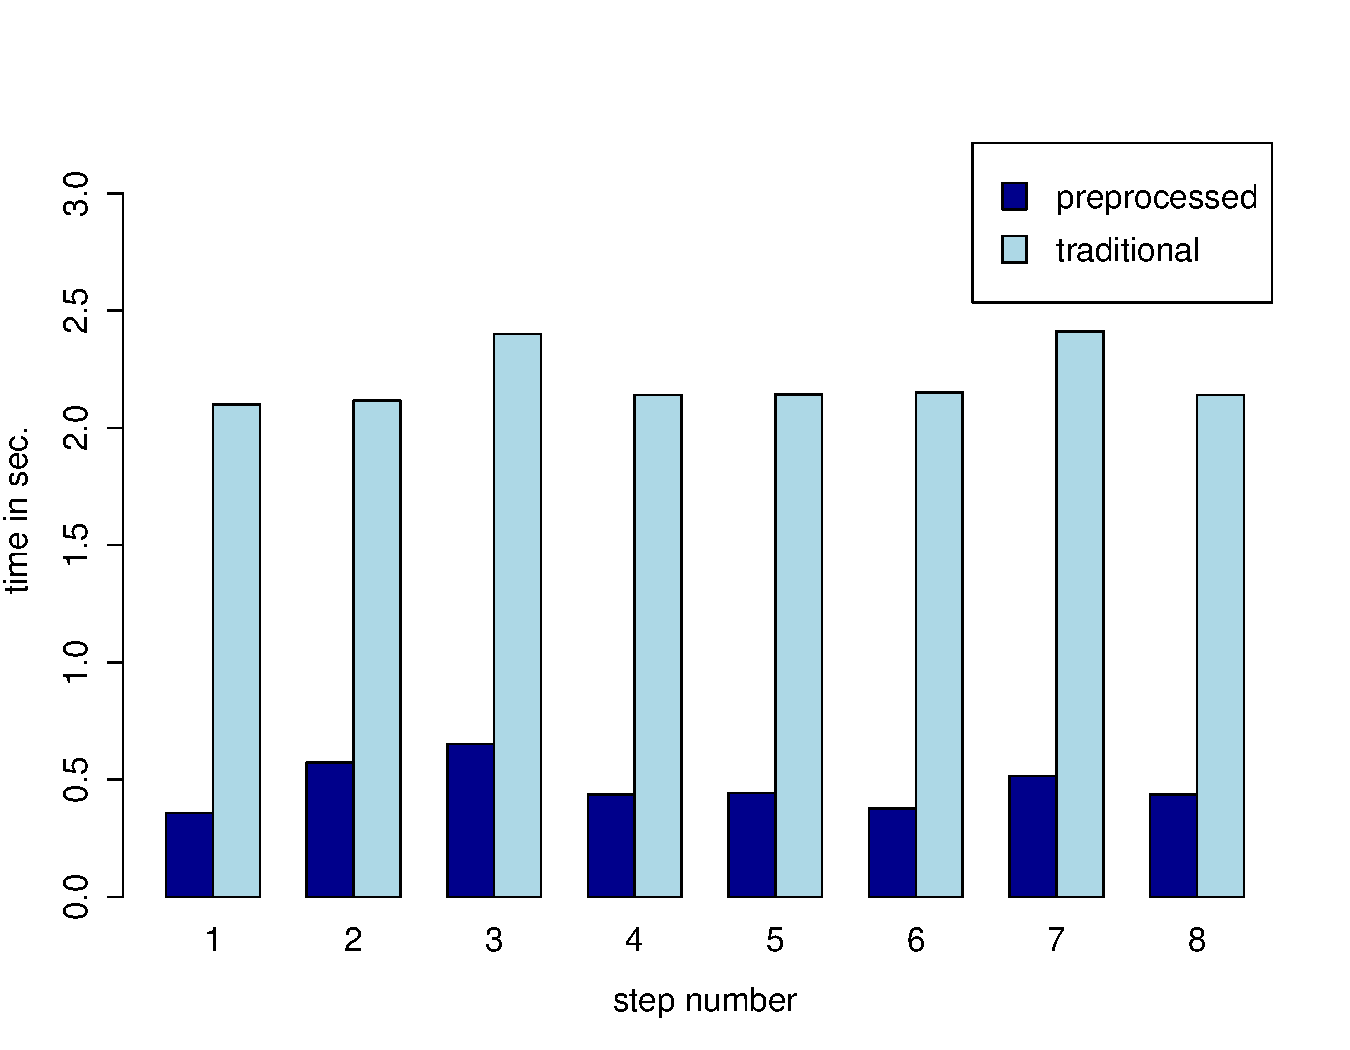
\includegraphics[width=0.5\textwidth]{Rplot26}
%     }
%   %  
%    % 
% %
% %
%     %}%\hfill
%     \subfloat[10 wards, reasoning time per event.\label{fig:results10ward}]{%
%       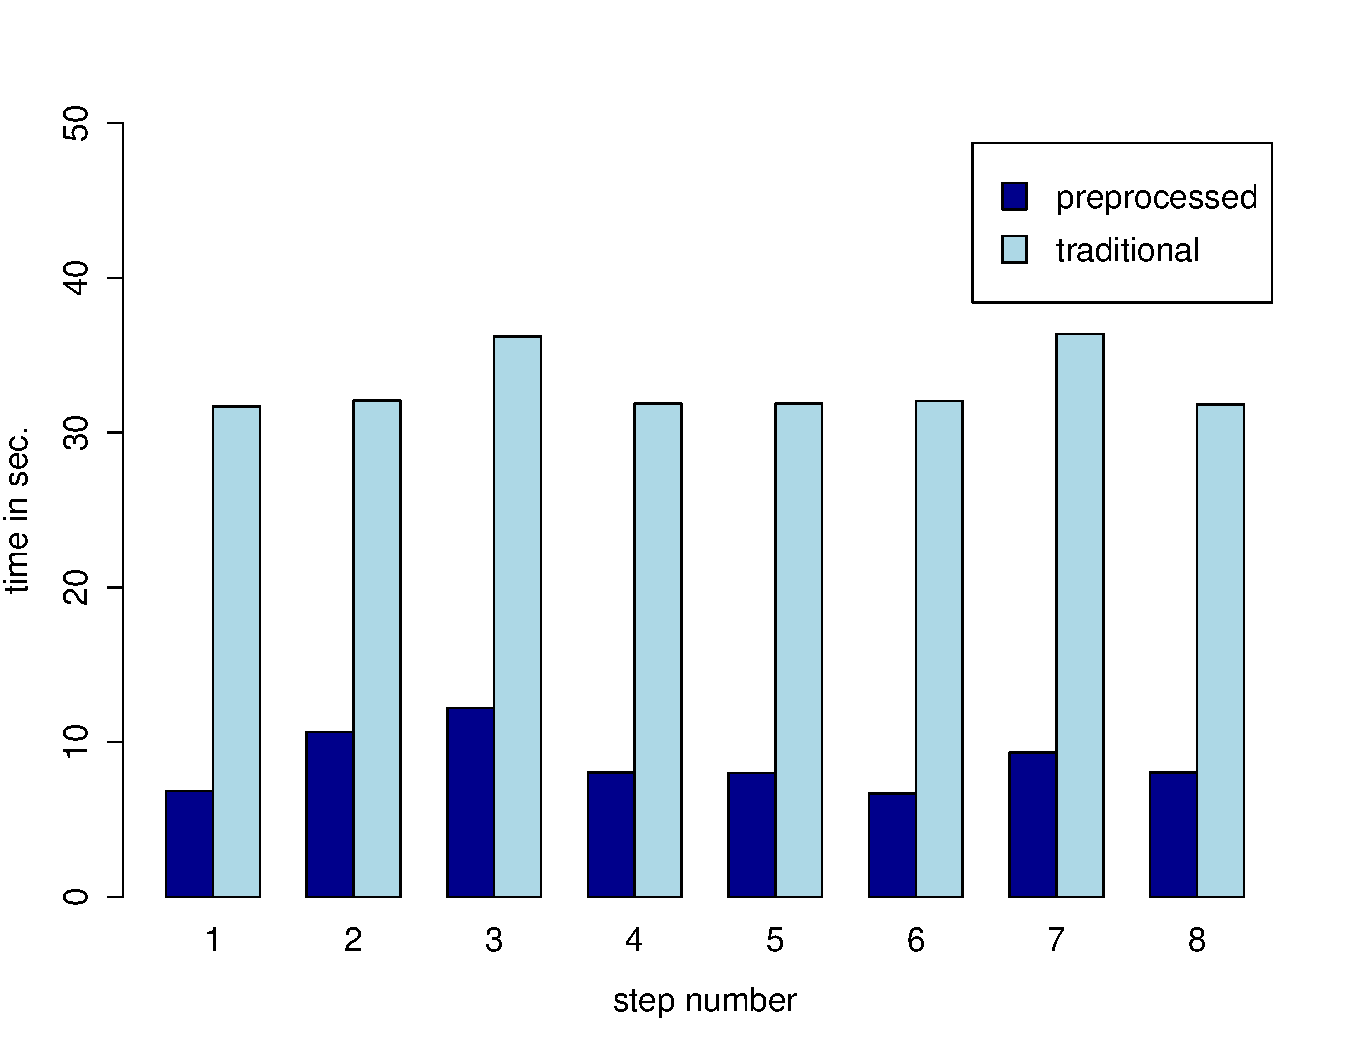
\includegraphics[width=0.5\textwidth]{Rplot27}
%     }
%     \caption{Comparison of reasoning times using preprocessed and traditional rules. The preprocessing step improves reasoning times.
%       }
%     \label{figure:results}
%   \end{figure}
%   
  

To better understand the impact of the preprocessing step, we further compare the reasoning times of the two implementations using \nthree. These are depicted 
in Figure~\ref{figure:results}.
The figure shows that preprocessing the rules improves reasoning times significantly,  consistently requiring only a quarter of the reasoning time.
This trend manifests itself regardless of the amount of dynamic data involved.
Whereas the traditional rule set can no longer be used in a hospital with 10 wards the 
preprocessed rule set still provides reasonable reasoning times. 
 \begin{figure}
\centering
\begin{subfigure}{.5\textwidth}
  \centering
  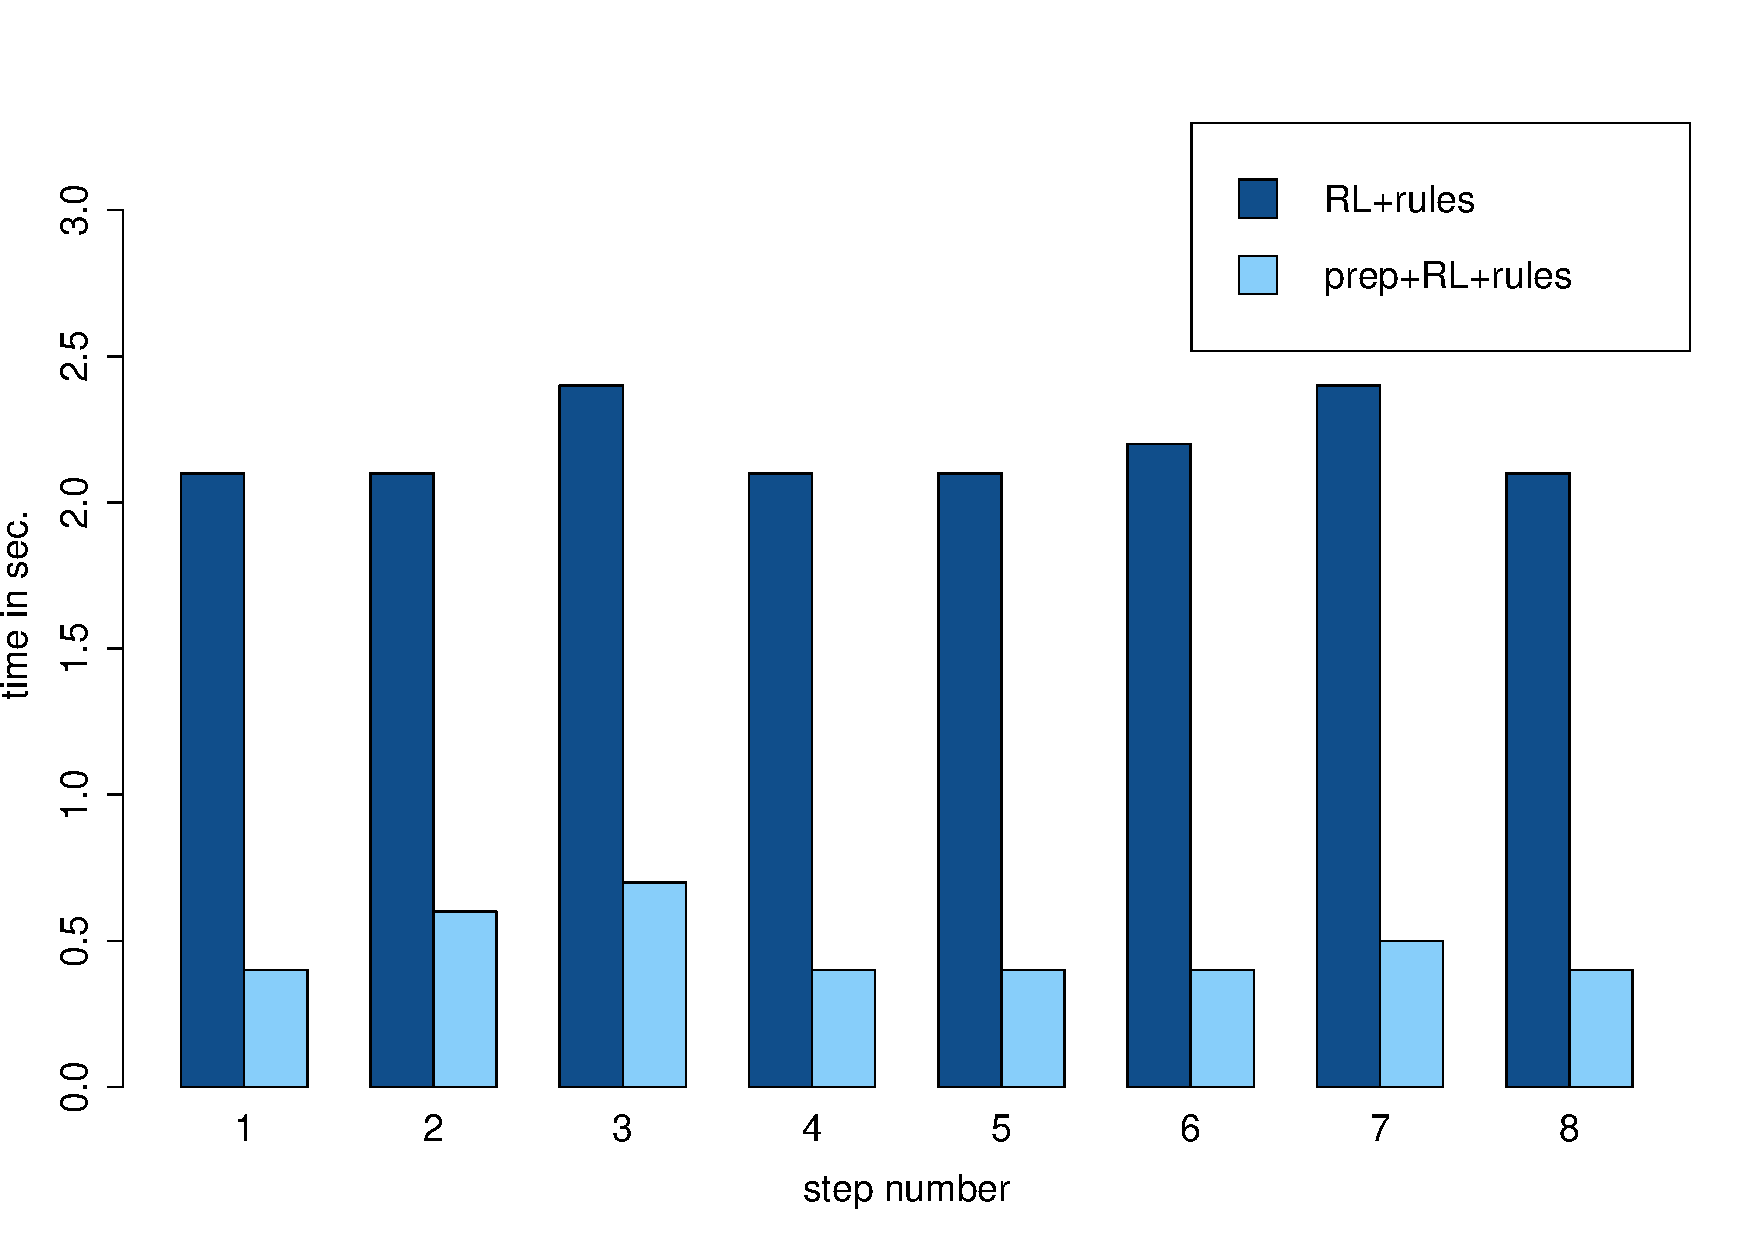
\includegraphics[width=\linewidth]{Rplot11}
  \caption{1 ward, reasoning time per event.}
  \label{fig:results1ward}
\end{subfigure}%
\begin{subfigure}{.5\textwidth}
  \centering
  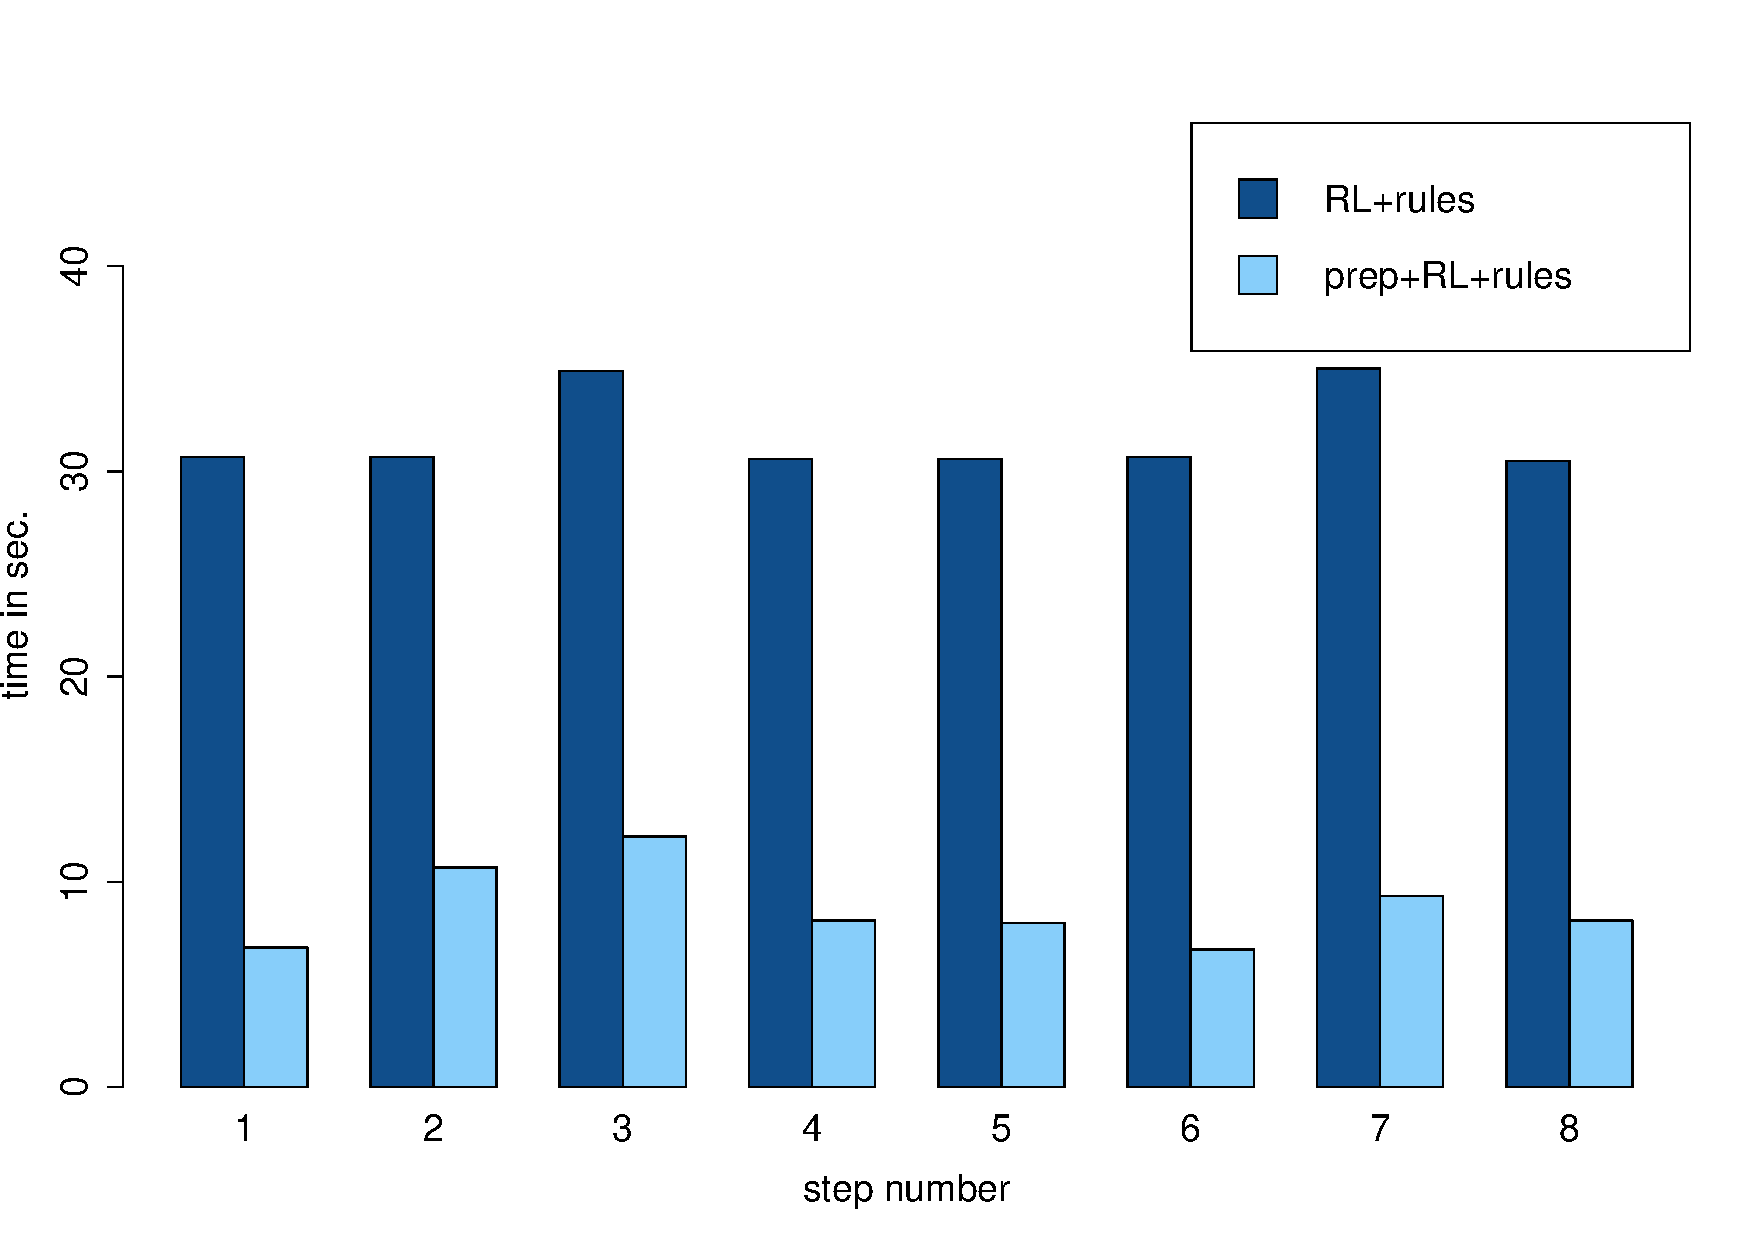
\includegraphics[width=\linewidth]{Rplot13}
  \caption{10 wards, reasoning time per event.}
  \label{fig:results10ward}
\end{subfigure}
\caption{Comparison of reasoning times using preprocessed and traditional RL rules in \nthree. The preprocessing step improves reasoning times.}
\label{figure:results}
\end{figure} 
 
\subsection{Discussion}
Our analysis has shown that the implementation using \owl RL and rules performs much faster than the one using OWL DL and SPARQL querying. The results could be 
further improved by using rule-producing rules, a special feature of \nthree. In this particular use case we can positively answer our initial question whether \nthree reasoning can 
solve the same practical problems as \owl DL reasoning and SPARQL querying with comparable performance. We can even say more: Here, the \nthree solutions outperform \owl DL and SPARQL.
But we also need to be careful: The OWL DL profile is of course more expressive than OWL RL and our good results were achieved by ignoring some derivations. 
In our use case these derivations were not relevant for the queries we wanted to answer and here we also see the actual advantage of using \nthree: We can customise the reasoning according to our needs.
From the various informations which are stated by means of an \owl DL ontology we chose which ones we wanted to use for further reasoning. If we need to be more expressive than \owl RL we can 
extend our rules set and use -- for example -- rules with new blank nodes in the consequent to support \owl ER \cite{owlex}, an \owl profile  which can be supported by existential rules. 
Powerful built-in functions provide us with even more options. By limiting the information we actually use for our conclusions, we can even reason over \owl Full ontologies 
and thereby accept an \owl format which is semantically compatible with \rdf.
% 
% 
% But these derivations 
% were not relevant for the queries we applied in our use case. Even though it was originally planned to solve the problem using OWL DL -- the ontology was created having this and 
% similar use cases in mind -- it was enough to only use OWL RL.  In our implementation we thereby chose which of the information available we want to use further snd here we also see the advantage 
% of using \nthree: OWL DL ontologies 

%semantic compatibility with \rdf.

% Above we compare the reasoning times of a very complex profile, \owl DL, with the less expressive profile \owl RL and it is therefore not surprising that the reasoning 
% is much faster.
% 
% I should say that we compared different things and that OWL DL is more expressive, but that the question here was rather focussed on practical cases and the conclusion we can draw is that we do not 
% always need OWL DL even when a solution was initially using that powerful profile. often, less expressive profiles are enough and these can be defined in a way which is semantically 
% compatible with \rdf.  